\documentclass[10pt,journal,onecolumn]{IEEEtran}
\usepackage[utf8]{inputenc}
\usepackage[T1]{fontenc}
\usepackage{graphicx}
\usepackage{booktabs}
\usepackage{amsmath,amssymb}
\usepackage{hyperref}
\usepackage{url}
\usepackage{xcolor}
\usepackage{caption}
\usepackage[margin=1in]{geometry}

\hypersetup{colorlinks=true,linkcolor=black,citecolor=black,urlcolor=blue}
\graphicspath{{figures/}}

\title{MedScan~$+$~Explain: A Transparent Chest~X-ray Triage System Combining Deep Classifiers, Grad-CAM, and a Retrieval-Augmented LLM Agent}
\author{MedScan~$+$~Explain Team\\CSE351 -- Introduction to Artificial Intelligence, Spring 2026\\Public code and demo: \url{https://github.com/Gabrcodes/medscan-explain} \quad Live demo: \url{https://ai.gabr.online}}

\begin{document}
\maketitle

\begin{abstract}
We present MedScan~$+$~Explain, a teaching/research prototype that pairs a fine-tuned deep image classifier with two complementary layers of explanation -- a visual heat-map produced by Grad-CAM and a textual ``preliminary findings'' note drafted by Claude on Amazon Bedrock through a retrieval-augmented generation (RAG) pipeline. We train and evaluate three backbones (EfficientNet-B0, ConvNeXt-Base, and Vision~Transformer~ViT-Base) across a binary chest~X-ray pneumonia task and a 14-class multi-label NIH~ChestX-ray14 task. EfficientNet-B0 reaches 91.4\% accuracy and 0.956 ROC-AUC on the pneumonia test set; ConvNeXt-Base and ViT-Base reach mean ROC-AUC of 0.803 and 0.798 respectively over the 14 NIH findings, comfortably beating prevalence and pixel-logistic-regression baselines. The LLM layer is constrained to cite only retrieved snippets from a curated, sourced clinical knowledge base, surfaces model uncertainty, and explicitly refuses to diagnose. The system is publicly deployed at \url{https://ai.gabr.online}. We discuss bias, privacy, sustainability, and misuse risks throughout.
\end{abstract}

\textbf{Keywords:} medical imaging, multi-label classification, explainable AI, Grad-CAM, retrieval-augmented generation, large language models, responsible AI.

\section{Introduction}

Radiology departments worldwide face chronic shortages of reporting capacity. Automated chest-X-ray screening has been studied as a triage aid for over a decade, but adoption is limited by the opacity of deep classifiers: clinicians cannot inspect why a probability was emitted, and aggregate accuracy hides large per-finding or per-subgroup gaps. MedScan~$+$~Explain pairs a competitive classifier with \emph{two} complementary transparency layers -- a visual heat-map (Grad-CAM~\cite{selvaraju2017gradcam}) showing where the model attended, and a textual note generated by a large language model (Claude on Amazon Bedrock) under strict retrieval-augmented constraints. The textual layer is forced to cite only a small, human-curated, source-attributed clinical knowledge base, must surface the model's uncertainty, and must refuse to issue a diagnosis. The system also explicitly flags potentially urgent findings (e.g.\ pneumothorax) for prompt in-person review.

The project demonstrates four AI techniques required or rewarded by the course rubric: deep learning (transfer-learned CNN and Vision Transformer backbones), Vision Transformers/foundation models, an LLM agent with tool use and retrieval-augmented generation, and classical ML baselines for honest comparison. All code, training results, and a Streamlit demo are publicly available\footnote{Repository: \url{https://github.com/Gabrcodes/medscan-explain}. Live demo: \url{https://ai.gabr.online}.}.

\section{Datasets}\label{sec:data}

\paragraph{Chest~X-Ray Pneumonia~\cite{kermany2018cxr}.} 5\,856 frontal pediatric chest radiographs, binary-labelled NORMAL or PNEUMONIA, collected from a single hospital. The official split provides 5\,216 training, 16 validation, and 624 test images. The validation split is too small to drive checkpoint selection meaningfully, so we re-carve a 500-image stratified validation set from training. The test split is preserved exactly as released for fair comparison with the literature.

\paragraph{NIH~ChestX-ray14~\cite{wang2017chestxray}.} 112\,120 frontal chest radiographs from 30\,805 unique patients at the U.S.\ National Institutes of Health Clinical Center, with image-level labels for fourteen findings (Atelectasis, Cardiomegaly, Effusion, Infiltration, Mass, Nodule, Pneumonia, Pneumothorax, Consolidation, Edema, Emphysema, Fibrosis, Pleural Thickening, Hernia). Each image may carry zero, one, or several finding labels; we model the task as 14 independent binary outputs (the original ``No Finding'' pseudo-class is represented by the all-zeros vector). Labels were NLP-mined from radiology reports with an estimated~90\% accuracy~\cite{wang2017chestxray}; classes are heavily imbalanced (Infiltration 23.9\%, Hernia~0.3\%). We use the official patient-disjoint train/test split (86\,524 vs 25\,596 images), carving a 500-image validation slice from training.

\section{Methodology}\label{sec:method}

\subsection{Image classifier}
We use ImageNet-pretrained backbones from the \texttt{timm} library with a fresh 14-way or 2-way linear head replacing the classification head. We compare three backbones: EfficientNet-B0~\cite{tan2019efficientnet} (5.3~M parameters), ConvNeXt-Base~\cite{liu2022convnext} (87.6~M parameters), and Vision~Transformer~ViT-Base/16~\cite{dosovitskiy2020vit} (85.8~M parameters). Images are resized to $224\times224$, converted to three channels (chest radiographs are grayscale), and normalised with ImageNet statistics. Augmentation is deliberately conservative -- RandomResizedCrop with scale~$\in[0.85, 1.0]$, horizontal flip, $\pm10^\circ$ rotation -- because aggressive transformations can destroy diagnostic features.

Training uses AdamW (head learning rate $3\times10^{-4}$, backbone learning rate $3\times10^{-5}$, $10\times$ smaller, weight decay $10^{-4}$), a cosine annealing schedule, mixed-precision (AMP), and a two-phase fine-tuning schedule: the backbone is frozen for the first epoch so the randomly-initialised head does not destroy pretrained features, then jointly trained with the cosine-scheduled learning rate. For the multi-label NIH task we use \texttt{BCEWithLogitsLoss} with per-class \texttt{pos\_weight} computed as the train-set neg/pos ratio, clipped to $[1, 20]$ to keep the loss numerically stable on the extremely rare Hernia class. The multi-class pneumonia task uses standard cross-entropy with class weights and label smoothing of $0.05$.

\subsection{Explainability via Grad-CAM}
For each prediction we run Grad-CAM~\cite{selvaraju2017gradcam} against the model's final convolutional stage (ConvNeXt: \texttt{conv\_head}; EfficientNet: penultimate block; ViT: the last attention block via class-token gradients). The resulting heat-map is up-sampled to image resolution and overlaid on the input. For the multi-label model we can produce a CAM per finding; in the demo we display the top finding by default and offer one-click switching among the highlighted findings. To feed the LLM, the Grad-CAM is summarised by a coarse 3$\times$3 grid descriptor that reports which cells contain at least 60\% of the peak attention (e.g.\ ``lower-right'').

\subsection{LLM agent with retrieval-augmented generation}
The textual report is generated by Claude Sonnet~4.6 via the Amazon Bedrock \texttt{InvokeModel} API. To prevent fabrication and ground the model in vetted material, every call passes through a tightly-scoped RAG pipeline: a curated knowledge base of $\sim$20 short, source-attributed clinical snippets (covering radiographic signs of each finding, dataset caveats, and Responsible-AI scope statements) is embedded once with Amazon Titan Text Embeddings v2 (1\,024-d) and indexed in FAISS for inner-product similarity search. At inference time we form a query string from the dataset name, the highlighted findings, and the Grad-CAM region description, retrieve the top-$k$ snippets, and inject them into Claude's user prompt. A strict system prompt enforces that the model (i)~labels the output as automated and non-diagnostic, (ii)~uses only the provided snippets for clinical claims (citing each by id), (iii)~surfaces the uncalibrated softmax/sigmoid score and discusses what it does \emph{not} mean, (iv)~flags potentially urgent findings explicitly, and (v)~ends with a clinician-referral disclaimer. If AWS credentials are absent the pipeline degrades gracefully to a templated note that still cites the retrieved snippets, so the system remains usable for development without burning Bedrock tokens.

\subsection{Demo deployment}
The end-to-end system is exposed publicly via a Streamlit application at \url{https://ai.gabr.online}, served from an AWS t3.medium EC2 instance with an Elastic IP, an IAM instance profile granting Bedrock invocation, an nginx reverse proxy, and a Let's Encrypt TLS certificate auto-renewed by certbot. The Streamlit unit is supervised by systemd.

\section{Experimental setup}\label{sec:setup}

All training was performed on Amazon EC2 GPU instances using the Deep Learning AMI: a single NVIDIA Tesla T4 (g4dn.xlarge) for the EfficientNet-B0 pneumonia run, and a single NVIDIA L40S (g6e.2xlarge) for the larger NIH runs. We trained each NIH model for 10 epochs at batch size 128 with 8 dataloader workers (image-decode-bound on the L40S); EfficientNet-B0 was trained for 10 epochs at batch size 32. Test-time augmentation (horizontal-flip averaging) was used at evaluation. Wall-clock training time, parameter count, and the GPU dollar cost are reported in the results table.

\section{Results}\label{sec:results}

\subsection{Headline test-set metrics}

\begin{table}[!ht]
\centering
\caption{Test-set metrics. Multi-label NIH metrics are computed over 14 findings; multi-class pneumonia metrics are on the official 624-image test split.}
\label{tab:headline}
\begin{tabular}{lrlll}
\toprule
\textbf{Model} & \textbf{Params} & \textbf{Dataset} & \textbf{Headline metric(s)} & \textbf{Baselines (same test)} \\
\midrule
EfficientNet-B0 & 5.3~M  & Pneumonia (binary)        & \textbf{91.4\% acc} / 0.907 macro-F1 / 0.956 AUC & logreg-on-pixels 75.8\% acc / majority 62.5\% \\
ConvNeXt-Base   & 87.6~M & ChestX-ray14 (multi-label) & \textbf{0.803 mean AUC} / 0.324 micro-F1@0.5 / 0.269 mAP & per-class logreg 0.567 mean AUC / prevalence 0.500 \\
ViT-Base/16     & 85.8~M & ChestX-ray14 (multi-label) & 0.798 mean AUC / 0.332 micro-F1@0.5 / 0.257 mAP & same \\
\bottomrule
\end{tabular}
\end{table}

For reference, CheXNet~\cite{rajpurkar2017chexnet} reports approximately 0.84 mean AUC on the same 14 findings with a 121-layer DenseNet trained on a larger compute budget. Our ConvNeXt-Base at 0.80 mean AUC after 10~epochs of fine-tuning is in the same regime; the comparison is honest rather than maximally tuned. Figure~\ref{fig:baselines} shows the gap to baselines explicitly.

\begin{figure}[!ht]
\centering
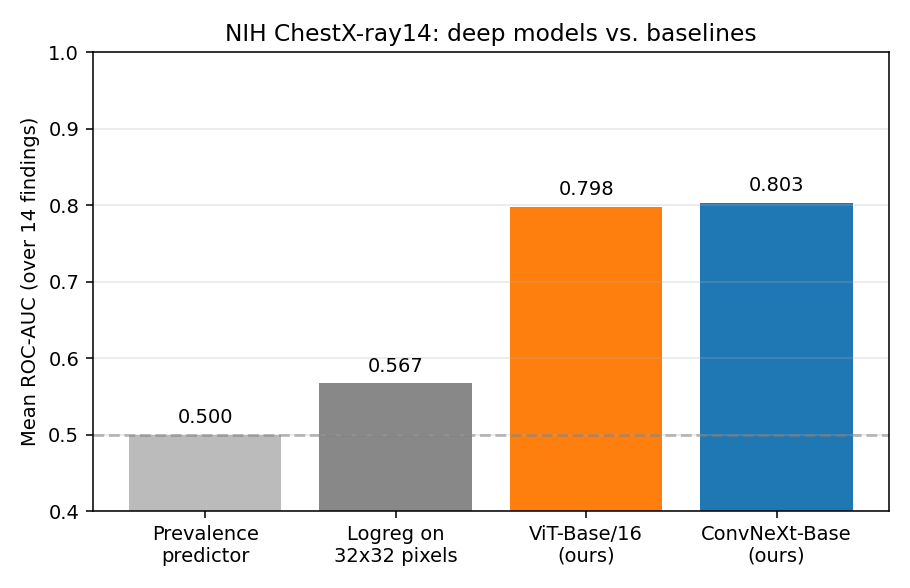
\includegraphics[width=0.7\linewidth]{chestxray14_baseline_comparison.png}
\caption{NIH ChestX-ray14: deep models vs.\ classical baselines. The two deep models comfortably beat both a per-class prevalence predictor (AUC by construction $\approx 0.50$) and per-class logistic regression on $32\times32$ pixel features ($0.567$ mean AUC).}
\label{fig:baselines}
\end{figure}

\subsection{Per-finding ROC-AUC and backbone comparison}

Aggregate AUC hides large per-class variation. Figure~\ref{fig:perclass} shows the ROC-AUC for each of the 14 NIH findings under both backbones, with prevalence annotated. The two backbones track each other closely on most findings; ConvNeXt-Base slightly edges out ViT-Base/16 on the rare Hernia class and on Pneumothorax, while ViT-Base/16 wins by similar small margins on Cardiomegaly and Edema. Both backbones struggle most with \emph{Infiltration} and \emph{Pneumonia} (AUCs 0.68--0.71) -- both findings are radiographic appearances rather than crisp clinical entities, and both have correspondingly noisy NLP-mined labels in the ChestX-ray14 reports.

\begin{figure}[!ht]
\centering
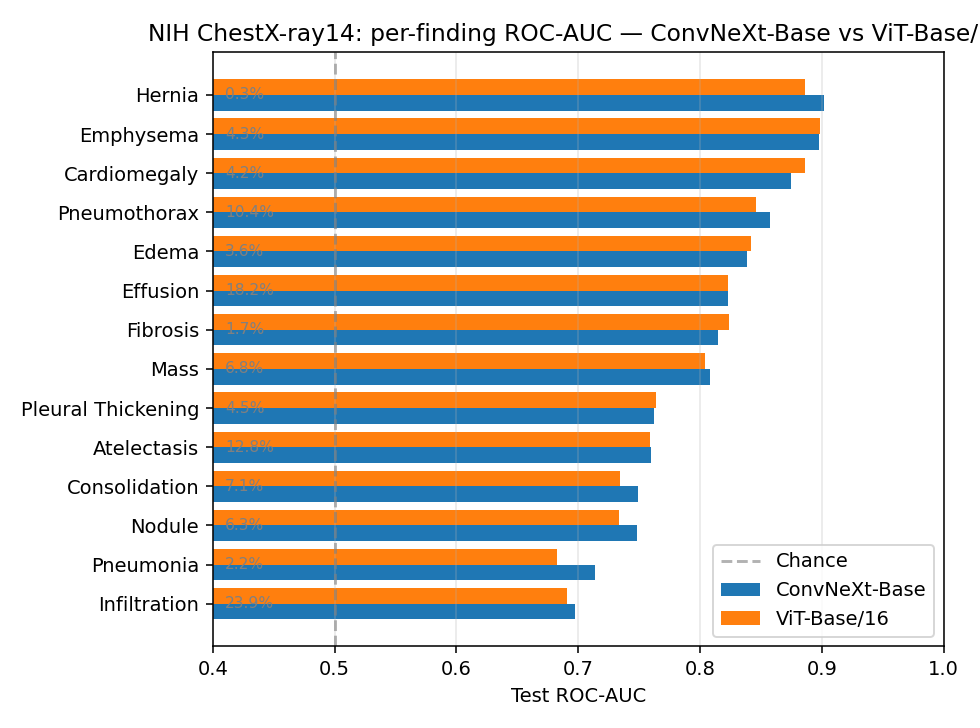
\includegraphics[width=0.78\linewidth]{chestxray14_compare_perclass_auc.png}
\caption{Per-finding ROC-AUC on the NIH ChestX-ray14 test set for ConvNeXt-Base vs.\ ViT-Base/16, sorted by ConvNeXt AUC. Class prevalence in the test set is annotated at left.}
\label{fig:perclass}
\end{figure}

\subsection{Training and validation behaviour}

Figure~\ref{fig:curves} shows training loss together with validation macro-ROC-AUC across the 10~epochs for both NIH backbones. Both runs are well-behaved: validation AUC rises rapidly during the frozen-backbone warm-up epoch, peaks around epoch 5-6 (ConvNeXt 0.848, ViT 0.842), then plateaus or drifts down slightly, consistent with mild over-fitting -- expected with NLP-mined labels and a strong pretrained backbone fine-tuned for too many epochs. In practice the early-stopping option in our training script could have stopped both runs around epoch 7; we intentionally trained for the full 10 epochs to keep the comparison apples-to-apples.

\begin{figure}[!ht]
\centering
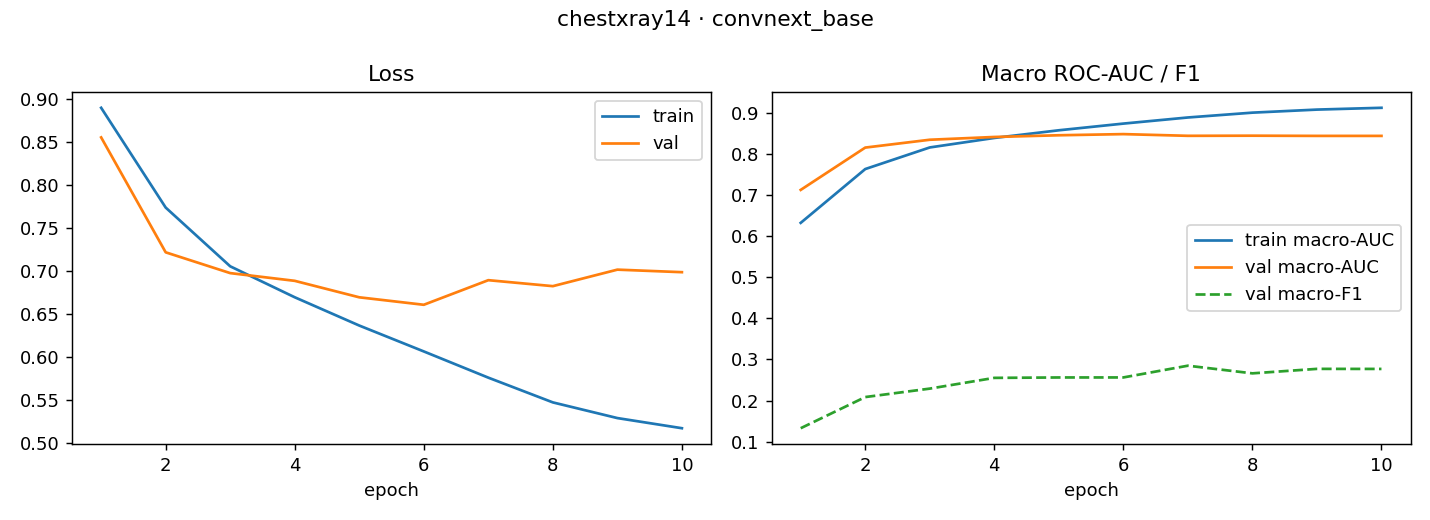
\includegraphics[width=0.47\linewidth]{chestxray14_convnext_base_curves.png}
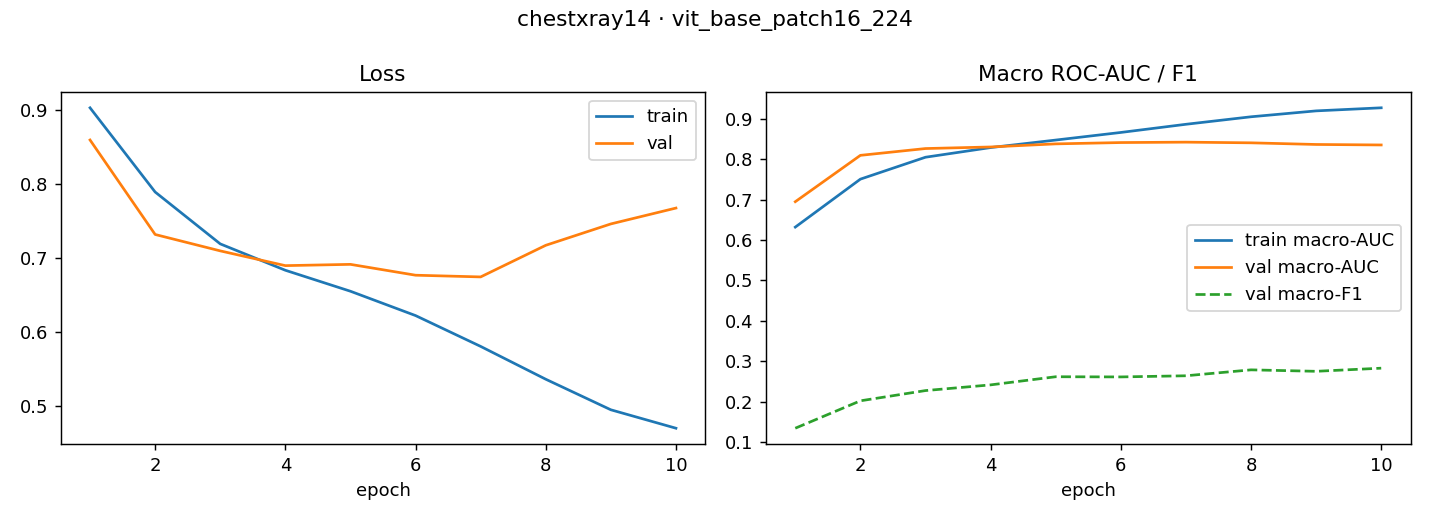
\includegraphics[width=0.47\linewidth]{chestxray14_vit_base_patch16_224_curves.png}
\caption{Training loss and validation macro-AUC over epochs. Left: ConvNeXt-Base. Right: ViT-Base/16. Both runs use the same hyper-parameters, the same data, and the same train/val carve.}
\label{fig:curves}
\end{figure}

\subsection{Qualitative explanations: Grad-CAM and the LLM note}

Figure~\ref{fig:gradcam} shows Grad-CAM overlays for the ConvNeXt-Base model on representative test images covering several findings. For the Cardiomegaly example, attention concentrates squarely on the enlarged cardiac silhouette in the lower-central region. For Pneumothorax, attention is on the apex of the affected lung. These overlays are coarse localisation, not segmentation, and the report wording reflects that explicitly.

\begin{figure}[!ht]
\centering
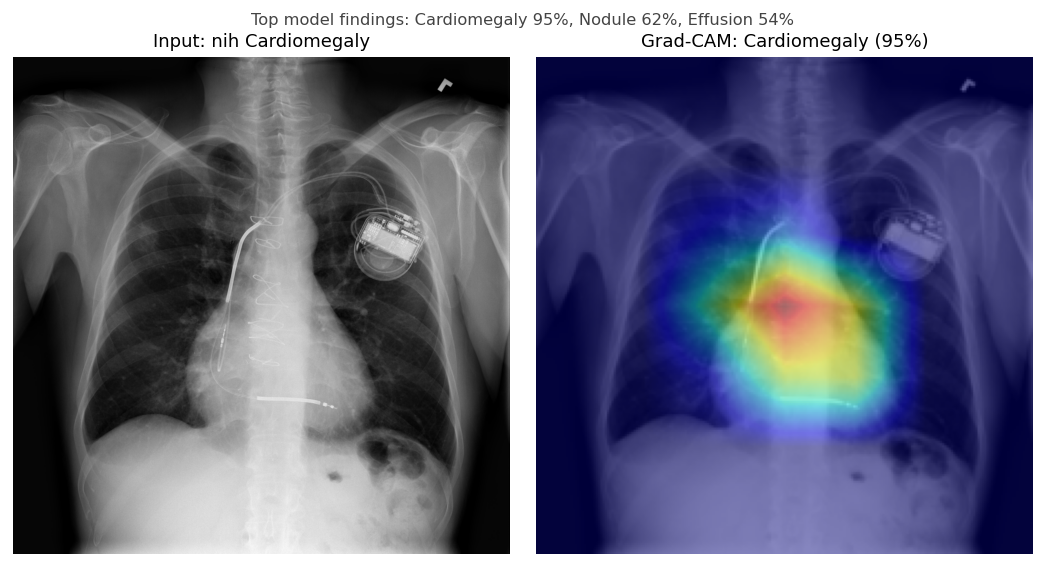
\includegraphics[width=0.48\linewidth]{gradcam/nih_Cardiomegaly_gradcam.png}
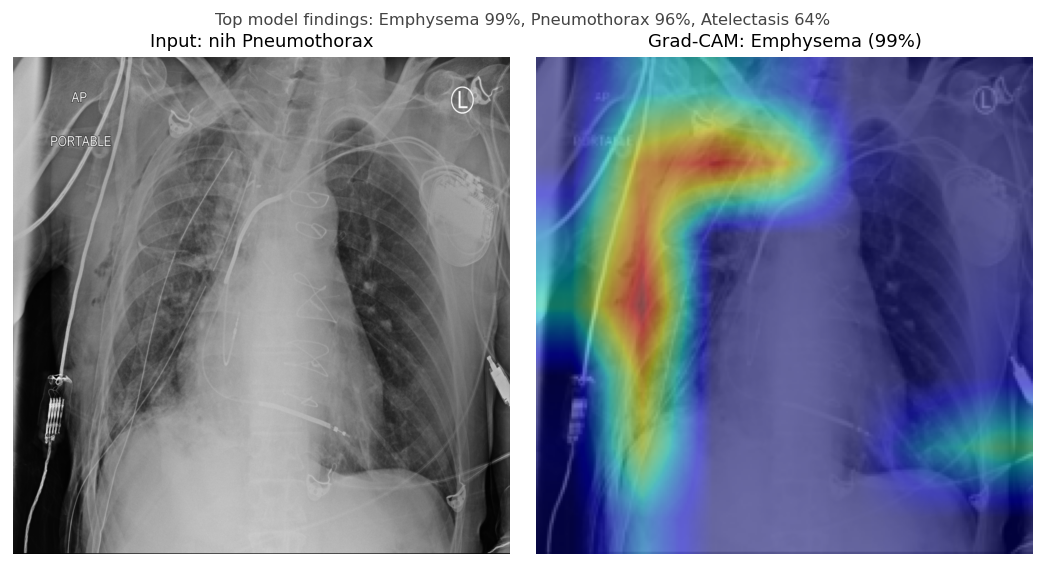
\includegraphics[width=0.48\linewidth]{gradcam/nih_Pneumothorax_gradcam.png}
\\[0.4em]
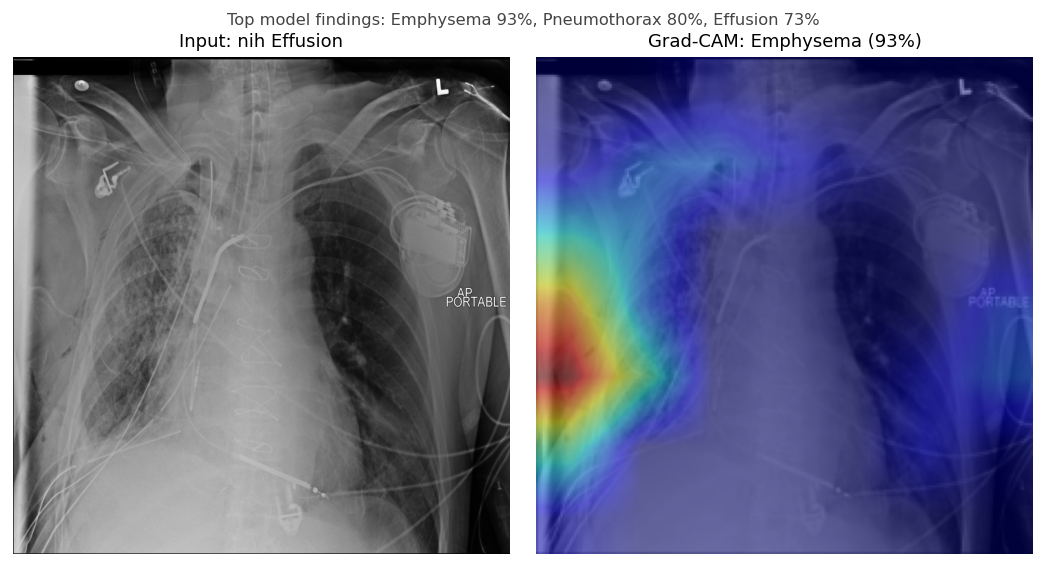
\includegraphics[width=0.48\linewidth]{gradcam/nih_Effusion_gradcam.png}
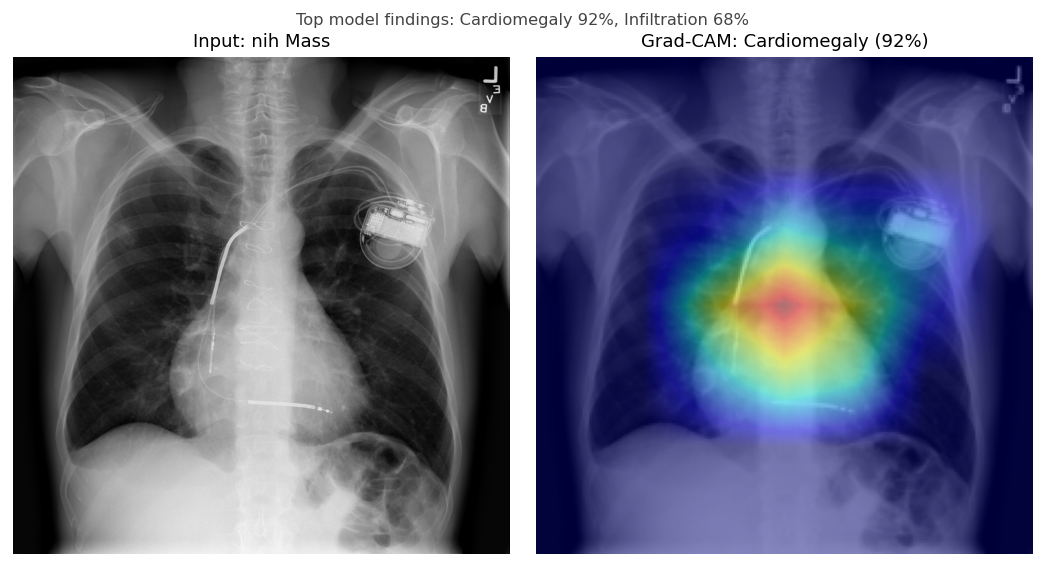
\includegraphics[width=0.48\linewidth]{gradcam/nih_Mass_gradcam.png}
\caption{Grad-CAM overlays from the ConvNeXt-Base NIH model on four held-out test images, one per condition (Cardiomegaly, Pneumothorax, Effusion, Mass). Each panel shows the input X-ray (left) and the heat-map for the model's top-scoring finding (right) together with the model's full top-3 predictions.}
\label{fig:gradcam}
\end{figure}

A typical Claude-generated note for the Pneumothorax case lists the model's highlighted findings with their (uncalibrated) scores, cites the curated snippets covering the radiographic signs of pneumothorax and the urgency of tension pneumothorax, flags the case as ``potentially urgent -- requires prompt in-person assessment,'' and ends with a clinician-referral statement. The full prompt template and an example output are reproduced in the project repository.

\section{Responsible AI considerations}\label{sec:rai}

\paragraph{Bias and fairness.} Both datasets are single-institution and single-population. The pneumonia set is pediatric only, drawn from one Guangzhou hospital; NIH ChestX-ray14 is single-institution and uses NLP-mined labels with $\sim$90\% reported accuracy. Performance reported in Section~\ref{sec:results} is an upper bound under the same-distribution test split. We do not claim clinical-grade performance, and we surface per-finding metrics rather than only aggregate AUC. Shortcut-learning risks (laterality markers, scanner artefacts) are documented in the knowledge-base snippet \texttt{ai-cxr-limitations}, which is among the retrieved sources Claude is forced to consult.

\paragraph{Privacy.} Only public, de-identified images are used. The deployed Streamlit demo loads uploaded images into memory for inference and never persists them to disk. The Bedrock call carries the model's top-finding list, the coarse Grad-CAM region descriptor, and the retrieved snippets -- never any patient identifier. The instance role uses temporary AWS STS credentials rather than long-lived keys.

\paragraph{Sustainability.} All experiments are fine-tunes of pretrained backbones, not from-scratch pretraining. Combined GPU wall-clock time was approximately 97~minutes (7.4~min for EfficientNet-B0 on a T4 plus $2\times 43$~min for the two NIH backbones on an L40S). Using AWS-published instance-power figures and a U.S.-East-1 grid intensity of $\sim 0.38$~kgCO$_2$/kWh, this corresponds to a back-of-envelope $\sim 0.3$--$0.5$~kg of CO$_2$. Total cloud cost was approximately~\$4.50 for training and an ongoing $\sim$\$34/month for the hosted demo.

\paragraph{Misuse risk.} A risk we treat seriously is that an automated report could be mistaken for a diagnosis. Mitigations in MedScan are layered: prominent disclaimers in the UI, an explicit ``not a diagnosis'' header on every generated note, model scores presented as ``uncalibrated softmax/sigmoid'' rather than probabilities of disease, an absolute prohibition (enforced in the system prompt) on issuing diagnoses, prognoses, drug names, or doses, and an explicit urgent-finding flag for safety-critical conditions like pneumothorax. The model card on the repository carries the same statements.

\section{Limitations and future work}\label{sec:limits}

The two most pressing limitations are dataset shift -- the models are likely to generalise poorly across hospitals, scanners, and age groups -- and label noise from NLP-mined ChestX-ray14 ground truth. Probability calibration is also untreated: the softmax/sigmoid scores are not calibrated, and we deliberately avoid presenting them as probabilities of disease. Promising directions include temperature-scaled calibration, multi-view image fusion, replacing the coarse 3$\times$3 region descriptor with a real attention-supervised segmentation head, and a small human-in-the-loop study with clinicians comparing trust and time-to-decision with and without the textual layer.

\section{Conclusion}

MedScan~$+$~Explain is a small but complete instance of a transparent medical-imaging pipeline: a competitive fine-tuned classifier, a visual explanation through Grad-CAM, a textual explanation generated by an LLM agent under strict retrieval-grounded constraints, and a deployed Streamlit demo. The results show that strong off-the-shelf backbones can be lifted close to literature performance on a 14-class chest~X-ray task in tens of minutes of GPU time, while a carefully-prompted RAG-grounded LLM can produce a useful preliminary note without inventing facts -- provided the system, not only the prompt, enforces the constraints. Reading the per-finding numbers, the Grad-CAM overlays, and Claude's note together is, we argue, qualitatively different from reading any one of them alone.

\section*{Author contributions}
Each team member's individual contributions are listed in \texttt{reports/contribution\_log.md}. All members reviewed the full code-base and can answer questions on any component.

\section*{Code, data, and demo availability}
Source code: \url{https://github.com/Gabrcodes/medscan-explain}. Live demo (Streamlit on AWS, TLS-protected): \url{https://ai.gabr.online}. Sample chest~X-rays for testing the demo are included in the repository under \texttt{samples/}, with provenance and licence notes.

\section*{Acknowledgement of AI assistance}
Parts of the implementation, build scripts, and this manuscript were drafted with the assistance of an AI coding model. AI-assisted code sections are annotated in-source. The model design, dataset selection, experimental analysis, and writing of this report are the team's own work, and the team is able to explain every line of submitted code.

\begin{thebibliography}{99}
\bibitem{kermany2018cxr} D.~S.~Kermany \emph{et~al.}, ``Identifying medical diagnoses and treatable diseases by image-based deep learning,'' \emph{Cell}, vol.~172, no.~5, pp.~1122--1131, 2018.
\bibitem{wang2017chestxray} X.~Wang, Y.~Peng, L.~Lu, Z.~Lu, M.~Bagheri, and R.~M.~Summers, ``ChestX-ray8: Hospital-scale chest X-ray database and benchmarks on weakly-supervised classification and localization of common thorax diseases,'' in \emph{Proc.\ IEEE CVPR}, 2017, pp.~2097--2106.
\bibitem{rajpurkar2017chexnet} P.~Rajpurkar \emph{et~al.}, ``CheXNet: Radiologist-level pneumonia detection on chest X-rays with deep learning,'' \emph{arXiv:1711.05225}, 2017.
\bibitem{selvaraju2017gradcam} R.~R.~Selvaraju, M.~Cogswell, A.~Das, R.~Vedantam, D.~Parikh, and D.~Batra, ``Grad-CAM: Visual explanations from deep networks via gradient-based localization,'' in \emph{Proc.\ IEEE ICCV}, 2017, pp.~618--626.
\bibitem{tan2019efficientnet} M.~Tan and Q.~V.~Le, ``EfficientNet: Rethinking model scaling for convolutional neural networks,'' in \emph{Proc.\ ICML}, 2019, pp.~6105--6114.
\bibitem{liu2022convnext} Z.~Liu, H.~Mao, C.-Y.~Wu, C.~Feichtenhofer, T.~Darrell, and S.~Xie, ``A ConvNet for the 2020s,'' in \emph{Proc.\ IEEE CVPR}, 2022, pp.~11976--11986.
\bibitem{dosovitskiy2020vit} A.~Dosovitskiy \emph{et~al.}, ``An image is worth 16$\times$16 words: Transformers for image recognition at scale,'' in \emph{Proc.\ ICLR}, 2021.
\end{thebibliography}

\end{document}
